\chapter{Design specification}\label{ch:design}

\section{Overview}

This section describes the design work done through the project as well as the tools used to carry that labor and the results of it. The chapter covers the following topics:

\begin{itemize}
\item \textbf{Architecture of the system:} The chosen architecture of the system is described, together with the reasons and advantages of the design.
\item \textbf{Design of the ontology:} The final design of the ontology is described, as well as it's advantages in front of other data modeling paradigms.
\item \textbf{Design of the central server:} The class design of the server is detailed in this section.
\item \textbf{Design of the web application:} The class design of the web application is detailed in this section, as well as the interface design.
\item \textbf{Design of the mobile application:} The class design of the mobile application is detailed in this section, as well as the interface design.
\item \textbf{Development environment:} The list of technologies employed in the project is detailed, briefly explaining the role of each tool.

\end{itemize}

\section{System architecture}\label{sec:designarch}

\begin{figure}[ht]
  \centering
  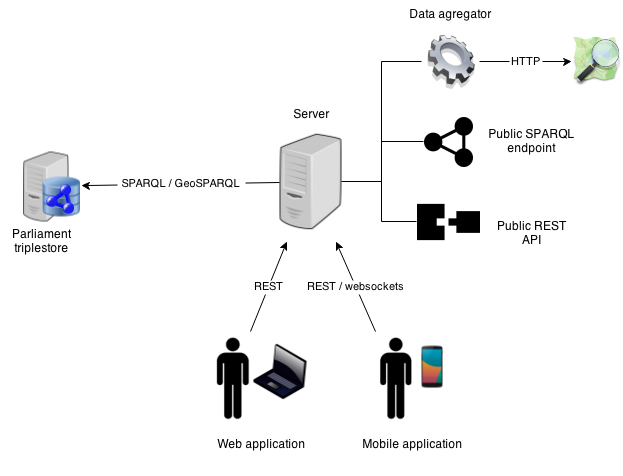
\includegraphics[width=.7\textwidth]{fig/architecture}
  \caption{Architecture design of the system}
  \captionsetup{font={footnotesize,bf,it}}
  \label{fig:architecture}
\end{figure} 

Figure \ref{fig:architecture} shows the architecture chosen for the system. This architecture comprises the following elements:

\begin{itemize}
\item A central server
  \begin{itemize}
  \item Web server
  \item SPARQL endpoint
  \item REST API
  \item Data agregator
  \item Database connector
  \end{itemize}
\item A semantic spatial storage system which contains the ontology
\item A web client used as the main interface of the system
\item A mobile application to support the browser based one
\end{itemize}

\subsection{Central server}

The central server is the core component of the system. It implements most of the functionality on the system and provides data to the client. It also analyzes the trails uploaded to the system and takes care of the communication with the database. The server is divided into several logical software pieces, which are described below.

\subsubsection*{Database connector}

The database connector implements the functionality needed to connect with the semantic data store. In essence, this means that it takes the requests from the users and transforms them into SPARQL queries. Then it takes the results provided by the database and converts them into a format that the server can process.

\subsubsection*{The data agregator}

This component has the function of querying external data sources and adapting the results to the data model of the system. It is independent of the rest of components of the server, since instead of being available to receive requests it will just run on demand. The component makes HTTP queries to the different APIs and endpoints on the web, for example OpenStreetMap and Geonames, and aggregates the data to the database.

\subsubsection*{REST API}

The API provides the basic means of accessing the information on the system. It is used by both clients to communicate with the server. It can be used for read, write and update operations, however, delete operations are not contemplated.

\subsubsection*{The SPARQL endpoint}

This endpoint just routes SPARQL queries done to it to the database. Its role is related to filtering the queries that seek to write and to ensure that no petition is going to break the integrity of the data in the database.

\subsection{Semantic spatial storage system}

This component of the system is mostly third party software. It consists on a triple store, a data storage system that stores RDF data; a reasoner supporting OWL and GeoSPARQL and an HTTP SPARQL endpoint. This component also englobes the ontology designed to define the data model of the system. This ontology is described in detail in section \ref{sec:ontdesign}.

\subsection{Web client}

The web client is the main interface though which the system is accessed. It communicates with the server through a REST API and offers most of the functionality of the system to the users.

The web application provides the usual functionality on web platforms, such as registering, browsing data, uploading data, editing the users profile and modifying data. Most of the operations have to be directly communicated to the server, however, there are certain functions such as the edition of trails that can be done offline and later uploaded to the server.

The client may be used from desktop browsers or mobile browser with no restrictions. More details on the design of the client can be found on section \ref{sec:webappdesign}.

\subsection{Mobile application}

The mobile client provides the functionality that the web application cannot. It offers real time functions by using a websocket API that the server exposes. If provides many of the browsing functionality of the web application on a interface adapted to be as mobile friendly as possible.

In addition, the mobile client exposes new functions typical of similar applications. These functions include the recording of a route and exporting it to a interchangeable format, that is GPX. In addition, the mobile application allows the creation of geolocated notes, which is not possible through the web application.

The design of this component is detailed in section \ref{sec:mobileappdesign}.

\subsection{Functioning of the system}

This section aims to provide an overview of how the system works and how the different components communicate among them.

The web and the mobile application will access the server through the API it exposes in every moment. The client will restrict the requests that can be sent to the server if the user is not logged in the system, however, for security reasons, the server will always check if the user is logged in the system if the operation modifies data.

All the requests result in a query to the semantic database. For this, the server creates a specific SPARQL query depending on the request done and sends it to the local URL where the endpoint is listening through an HTTP request. Then, the server parses the response, transforms it to a regular JSON object and replies it to the client.

The normal flow of information on the system is as follows: 

\begin{enumerate}
\item The client sends a request to the server
\item The server performs some operations and sends a request to the data store
\item The data store answers and the server parses the request into a JSON file
\item The data is returned to the client
\item The client uses the data
\end{enumerate}

However, there is an exception to this flow when exercising real time communication in the mobile application. In this case, there is not always a response to the client. Since this communication is done through a persistent connection, the flow of information is the following:

\begin{enumerate}
\item The client establishes a connection
\item The client sends its coordinates to the server
\item The server queries the database for nearby features
\item The server checks if there is any new information compared to the previous requests
\item If there is new information, the server replies only with the new data, if there is not there is not response
\end{enumerate}

In any case, the client will send periodic responses without worrying if the server actually responds or not.

\FloatBarrier
\section{Design of the ontology}\label{sec:ontdesign}

The ontology designed in the project represents specific knowledge related to the domain of Trails, Points of Interest and GPS data in general. It uses external ontologies as a base, in order to ease the sharing of information and the publishing of the dataset at Linked Open Data.

\begin{figure}[ht]
  \centering
  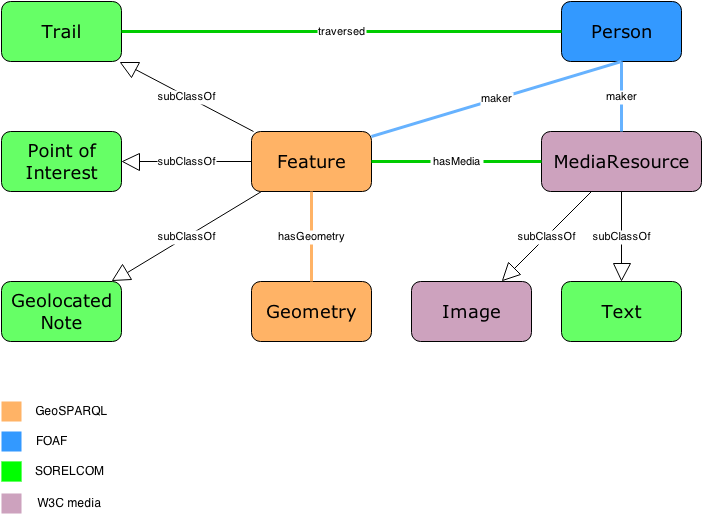
\includegraphics[width=.8\textwidth]{fig/sorelcom-ontology}
  \caption{The SORELCOM ontology}
  \captionsetup{font={footnotesize,bf,it}}
  \label{fig:sorelcom-ontology}
\end{figure} 

Figure \ref{fig:sorelcom-ontology} provides a graphical representation of classes on the SORELCOM ontology. As shown on the figure, classes from four vocabularies are reused. The FOAF vocabulary is used to obtain a representation of the users of the platform, the GeoSPARQL vocabulary is used as a base for all the resources with a spatial character , the W3C media vocabulary is used to represent the media resources on the platform and the Review vocabulary, representing the reviews and comments done by the users.

The focus of the design is to reuse as many well known vocabularies as possible and defining the needed classes, relations and properties to satisfy the requirements of the ontology 4 to 10, defined in chapter \ref{ch:requirements}.

\subsection{Class hierarchy}

The ontology defines a series of classes for the representation of specific spatial features present in the domain of the application. The classes are listed below:

\begin{description}
\item[\texttt{sorelcom:Trail}] A trail represents a path in the world. In the context of the application, a trail can be interpreted as a path that a user has traversed or as a simple route that is indicated by a user, however, the ontology does not specify that a trail should have any of these meanings.

\item[\texttt{sorelcom:PointOfInterest}] A Point of Interest is a feature in the world that may result of some interest for a person. There is no specification on what can be the interest a person may have on the feature, thus a point of interest may be anything from a monument to a restaurant.

\item[\texttt{sorelcom:GeolocatedNote}] A Geolocated Note is a message with a spatial context. This message is left by a person at a specific location, and can be viewed by any person or just a specific group depending on its privacy settings. The message on a note may be formed by text, images, video or any combination of them.

\item[\texttt{sorelcom:Category}] A category used to classify the types of point of interest. Categories contain a human readable name, a depiction and a description.

\end{description} 

In addition to the core types on the vocabulary, other classes obtained from external ontologies will be used or extended to represent different types of resources on the ontology. The additional classes used are the following:

\begin{description}
\item[\texttt{foaf:Person}] This class is used to classify resources as persons. Any user on the system will be classified as person. The class is defined in the FOAF vocabulary.

\item[\texttt{geo:Feature}] A feature is any object in the real world that has a spatial representation. \textit{Trails}, \textit{Points of Interest} and \textit{Geolocated Notes} are all types of Features. This class is defined in the GeoSPARQL vocabulary.

\item[\texttt{geo:Geometry}] In the GeoSPARQL ontology, a geometry is used to give a spatial representation to a Feature. Without a associated feature, geometries are not resources on the real world.

\item[\texttt{media:MediaResource}] A media resource is a representation of a media object, such as a image or a video. Media resources refer to the images, posts and videos saved in the system.

\item[\texttt{media:Image}] A image is a specialized media resource, which refers to a image. 

\item[\texttt{rev:Review}] A review of a resource. Used for the representation of user posts on the features of the system. It may include comments, ratings or both.
 
\end{description}

\subsection{Properties}

Most of the work on the design of the ontology consists on the creation of properties which relate the resources to the information that they must contain. Still, many of the properties used in the data model of the platform are obtained from external vocabularies.

Namespace notation is used to represent external ontologies. The relation of vocabularies, their namespaces and the URIs they represent is shown in table \ref{tab:namespaces}.

The properties and classes are represented by a IRI. This IRI is just the namespace appended with the class or property name. For example, foaf:name and http://xmlns.com/foaf/0.1/name are equivalent. 

\begin{table}[ht]
  \centering
  \caption{Points of interest on the SORELCOM data model.}\label{tab:namespaces}
  \begin{tabular}{lll}
    \toprule
      \textbf{Ontology} & \emph{namespace}  & \emph{URI}\\
    \midrule
       SORELCOM & sorelcom & http://morelab.deusto.es/ontologies/sorelcom \\
       FOAF & foaf & http://xmlns.com/foaf/0.1/ \\
       GeoSPARQL & geo & http://www.opengis.net/ont/geosparql\#\\
       W3C media & ma & http://www.w3.org/ns/ma-ont\\
       Review & rev & http://purl.org/stuff/rev\\
       Dublin Core & dcterms & http://purl.org/dc/elements/1.1/\\
       RDF & rdf & http://www.w3.org/1999/02/22-rdf-syntax-ns\#\\
       RDF schema & rdfs & http://www.w3.org/2000/01/rdf-schema\#\\
       OWL & owl & http://www.w3.org/2002/07/owl\#\\
    \bottomrule
  \end{tabular}
\end{table}

The properties defined for the SORELCOM vocabulary are listed below, together with a table representing how the information about those resources is stored in the data model:

\subsubsection*{Feature properties}

\begin{description}
\item[\texttt{sorelcom:name}] Property representing the human readable name of a feature. 
\item[\texttt{sorelcom:description}] Property representing a textual description of a feature.
\item[\texttt{sorelcom:hasMedia}] Property relating a feature to the media associated. It is the inverse of \texttt{sorelcom:mediaOf}.
\end{description}

\subsubsection*{Trail properties}

\begin{description}
\item[\texttt{sorelcom:difficulty}] Property representing the difficulty score of a trail. This score is a integer from 0 to 100, the higher the difficulty the higher the number. A trail may only have one difficulty.
\item[\texttt{sorelcom:maximumAltitude}] Property representing the altitude of the highest point of a trail.
\item[\texttt{sorelcom:minimumAltitude}] Property representing the altitude of the lowest point of a trail.
\item[\texttt{sorelcom:totalDistance}] Property representing the total distance in meters that must be traversed from the starting point of a trail to the end of it.
\item[\texttt{sorelcom:ascendingDistance}] Property representing the sum of the distance in meters of the segments of the trail which are ascendant .
\item[\texttt{sorelcom:descendingDistance}] Property representing the sum of the distance in meters of the segments of the trail which are descendant.
\item[\texttt{sorelcom:circular}] Property representing if the starting point and end point of a trail are the same.
\item[\texttt{sorelcom:traversedBy}] Property relating a trail to the users who have traversed it.
\end{description}

Information about how trails are represented on the system can be found on table \ref{tab:trail}.

\begin{table}[ht]
  \centering
  \caption{Trails on the SORELCOM data model.}\label{tab:trail}
  \begin{tabular}{llll}
    \toprule
      \textbf{Property} & \emph{domain}  & \emph{range} & \emph{information}\\
    \midrule
      sorelcom:name & geo:Feature  & string & name \\
      sorelcom:description & geo:Feature & string  & description \\
      sorelcom:difficulty & sorelcom:Trail & integer & difficulty \\
      sorelcom:maximumAltitude & sorelcom:Trail & float & maximum altitude \\
      sorelcom:minimumAltitude & sorelcom:Trail & float & minimum altitude \\
      sorelcom:ascendingDistance & sorelcom:Trail & integer & ascending distance \\
      sorelcom:descendingDistance & sorelcom:Trail & integer & descending distance \\
      sorelcom:hasMedia & geo:Feature & ma:Media & images and videos \\
      foaf:maker & Thing & foaf:Person & author \\
      sorelcom:traversedBy & sorelcom:Trail & foaf:Person & persons who traversed it \\ 
      geo:hasGeometry & geo:Feature & geo:Geometry & spatial representation \\
      rev:hasReview & rdfs:Resource & rev:Review & posts \\
    \bottomrule
  \end{tabular}
\end{table}

\subsubsection*{Point of interest properties}

\begin{description}
\item[\texttt{sorelcom:altitude}] Property representing altitude of the point. 
\item[\texttt{sorelcom:category}] Property representing the category of the point of interest.
\end{description}

Information about how points of interest are represented on the system can be found on table \ref{tab:poi}.

\begin{table}[ht]
  \centering
  \caption{Points of interest on the SORELCOM data model.}\label{tab:poi}
  \begin{tabular}{llll}
    \toprule
      \textbf{Property} & \emph{domain}  & \emph{range} & \emph{information}\\
    \midrule
      sorelcom:name & geo:Feature  & string & name \\
      sorelcom:description & geo:Feature & string  & description \\
      sorelcom:altitude & sorelcom:PointOfInterest & float & altitude \\
      sorelcom:category & sorelcom:PointOfInterest & sorelcom:Category & category \\
      sorelcom:hasMedia & geo:Feature & ma:Media & images \\
      foaf:maker & Thing & foaf:Person & author \\
      geo:hasGeometry & geo:Feature & geo:Geometry & spatial data \\
      rev:hasReview & rdfs:Resource & rev:Review & posts \\
    \bottomrule
  \end{tabular}
\end{table}

\subsubsection*{Geolocated Note properties}

\begin{description}
\item[\texttt{sorelcom:range}] Property representing range of action of a Geolocated Note. 
\item[\texttt{sorelcom:public}] Property representing if the note is public.
\item[\texttt{sorelcom:targets}] Property relating the note to the persons that should receive it. It exists only when the note is not public.
\end{description}

Information about how geolocated notes are represented on the system can be found on table \ref{tab:note}.

\begin{table}[ht]
  \centering
  \caption{Geolocated notes on the SORELCOM data model.}\label{tab:note}
  \begin{tabular}{llll}
    \toprule
      \textbf{Property} & \emph{domain}  & \emph{range} & \emph{information}\\
    \midrule
      dcterms:created & Thing & date & creation time \\
      dcterms:valid & Thing & date or integer & duration \\
      sorelcom:description & geo:Feature & string & textual content \\
      sorelcom:public & sorelcom:GeolocatedNote & boolean & privacy level \\
      sorelcom:radius & sorelcom:GeolocatedNote & integer & action radius \\
      sorelcom:hasMedia & geo:Feature & ma:Media & text, multimedia \\
      foaf:maker & Thing & foaf:Person & author \\
      geo:hasGeometry & geo:Feature & geo:Geometry & spatial representation \\
    \bottomrule
  \end{tabular}
\end{table}

\subsubsection*{Person properties}

\begin{description}
\item[\texttt{sorelcom:hasTraversed}] Property relating a Person to the trails it has traversed.
\item[\texttt{sorelcom:trailBuddyOf}] Property relating a Person to his/her trail buddies.
\end{description}

Information about how persons are represented on the system can be found on table \ref{tab:user}.

\begin{table}[ht]
  \centering
  \caption{Persons on the SORELCOM data model.}\label{tab:user}
  \begin{tabular}{llll}
    \toprule
      \textbf{Property} & \emph{domain}  & \emph{range} & \emph{information}\\
    \midrule
      foaf:nick & foaf:Person  & string & nickname \\
      foaf:mbox & foaf:Person  & string & email \\
      foaf:firstName & foaf:Person  & string & first name \\
      foaf:familyName & foaf:Person  & string & family name \\
      foaf:depiction & foaf:Person  & foaf:Image & avatar \\
      sorelcom:trailBuddyOf & foaf:Person  & foaf:Person & trail buddies \\
      sorelcom:hasTraversed & foaf:Person & sorelcom:Trail & traversed trails \\
      foaf:weblog & foaf:Person  & URI & external homepage \\
      foaf:made & foaf:Person  & Thing & features and media \\
    \bottomrule
  \end{tabular}
\end{table}

\subsubsection*{Media properties}

\begin{description}
\item[\texttt{sorelcom:mediaOf}] Property relating a media resource to the feature it belongs to.
\end{description}

Information about how media resources are represented on the system can be found on table \ref{tab:media}. Media resources are divided into images and video, however, for convenience purposes both of them are presented in a single table. 

\begin{table}[ht]
  \centering
  \caption{Media on the SORELCOM data model.}\label{tab:media}
  \begin{tabular}{llll}
    \toprule
      \textbf{Property} & \emph{domain}  & \emph{range} & \emph{information}\\
    \midrule
      foaf:maker & Thing & foaf:Person & author \\
      ma:description & ma:MediaResource & string & content \\
      ma:locator & ma:MediaResource & URI & download link \\
      dcterms:created & Thing & datetime & addition date \\
      sorelcom:mediaOf & ma:MediaResource & geo:Feature & feature \\
    \bottomrule
  \end{tabular}
\end{table}

\subsubsection*{Review properties}

Information about the representation of reviews an be found on table \ref{tab:review}. Reviews are formed by a rating of the feature and a possible textual comment on it. All properties used for review representation and relation are external.

\begin{table}[ht]
  \centering
  \caption{Posts on the SORELCOM data model.}\label{tab:review}
  \begin{tabular}{llll}
    \toprule
      \textbf{Property} & \emph{domain}  & \emph{range} & \emph{information}\\
    \midrule
      rev:reviewer & rev:Review & foaf:Person & author \\
      rev:text & rev:Review & string & textual content \\
      rev:rating & rev:Review & integer & user evaluation \\
      sorelcom:mediaOf & ma:MediaResource & geo:Feature & feature \\
      dcterms:created & Thing & datetime & creation date \\
    \bottomrule
  \end{tabular}
\end{table}

\subsubsection*{Category properties}

Categories are not specified by any requirement, however a representation for them is created in order to provide information about these categories and what they represent to the user. Information about these resources can be found in table \ref{tab:category}.

\begin{table}[ht]
  \centering
  \caption{Categories on the SORELCOM data model.}\label{tab:category}
  \begin{tabular}{llll}
    \toprule
      \textbf{Property} & \emph{domain}  & \emph{range} & \emph{information}\\
    \midrule
      rdfs:label & rdfs:Resource & string & name \\
      rdfs:comment & rdfs:Resource & string & description \\
      foaf:depiction & Thing & foaf:Image & icon representation \\
    \bottomrule
  \end{tabular}
\end{table}

\subsection*{Inference mechanism}

In order to get the maximum benefit from the semantic dataset the ontology has been defined using OWL. Due to this, several inference mechanism have been available during the design process, however, only a subset of them have been used. The following inference mechanisms have been used:

\begin{description}
\item[Sub classes] All resources which are instanced of a certain class A are also instances of the classes A is subclass of. This property is provided by RDF schema (see section \ref{sec:rdf} for more information). In RDF it is possible to use multiple inheritance, meaning that a class can be subclass of more than one class.
\item[Disjoint classes] A group of disjoint classes indicate that a resource of one class of the group cannot be of another class on the group
\item[Sub properties] Subproperty relations are the analogous of subclass relations when referring to resources of type property. It is also provided by RDF schema.
\item[Function properties] A functional property is a property that can only appear once in the triples of a certain resource. It is provided by OWL lite.
\item[Inverse properties] When a resource A is related to B by a property P1, then B is related to A by the property P2 inverse of P1. It is provided by OWL lite.
\item[Symmetric property] When a resource A is related to B by a symmetric property P, then B is related to A also by P.

\end{description}

Table \ref{tab:inferencecls} shows the inference rules used on the classes of the ontology and \ref{tab:inferenceprop} shows the inference rules used on the properties of the data model.

\begin{table}[ht]
  \centering
  \caption{Inferences used on the SORELCOM ontology classes.}\label{tab:inferencecls}
  \begin{tabular}{llll}
    \toprule
      \textbf{Class} & \emph{inference type}  & \emph{Related class}\\
    \midrule
      sorelcom:Trail & subclass of & geo:Feature \\
      sorelcom:PointOfInterest & subclass of & geo:Feature \\
      sorelcom:GeolocatedNote & subclass of & geo:Feature \\
      sorelcom:Text & subclass of & ma:MediaResource \\
      sorelcom:Trail & disjoint with & sorelcom:PointOfInterest \\
      sorelcom:Trail & disjoint with & sorelcom:GeolocatedNote \\
      sorelcom:GeolocatedNote & disjoint with & sorelcom:PointOfInterest \\
    \bottomrule
  \end{tabular}
\end{table}

\begin{table}[ht]
  \centering
  \caption{Inferences used on the SORELCOM ontology classes.}\label{tab:inferenceprop}
  \begin{tabular}{llll}
    \toprule
      \textbf{Property} & \emph{inference type}  & \emph{Related property}\\
    \midrule
      sorelcom:trailBuddyOf & sub property of & foaf:knows \\
      sorelcom:trailBuddyOf & symmetric property \\
      sorelcom:hasTraversed & inverse property of & sorelcom:traversedBy \\
      sorelcom:hasMedia & inverse property of & sorelcom:mediaOf \\
      sorelcom:difficulty & functional property \\
      sorelcom:maximumAltitude & functional property \\
      sorelcom:minimumAltitude & functional property \\
      sorelcom:totalDistance & functional property \\
    \bottomrule
  \end{tabular}
\end{table}

\subsection{Advantages of ontology based design}

The data model on the platform has been designed based on a ontology, mainly to follow the best practices of Linked Open Data. However, there are other alternatives, for instance, using a relational database and a RDF mapper. Mappers, for example, D2RQ expose the data on a relational database as a virtual RDF graph, allowing to query this data using SPARQL. This mappers exist to allow Semantic Web application to access the information stored on relational systems \cite{d2rq}.

Even with this alternatives, the choice to use a completely semantic system over a relational database was made. This choice came with some disadvantages, the main of them being an increased of the complexity of the system. RDF lacks support on programming platforms compared to relational database systems, thus the amount of coding needed increases. Besides, the current standard for the creation of GIS systems, the PostGIS \cite{postgis} extension for the PostgreSQL \cite{postgres} cannot be used. The rest of the spatial databases, including the semantic ones lack support and tools to work with, which has caused an increase in development times.

However using ontologies to define the data model of the platform brings several benefits. The main benefits are detailed in this section.

\subsubsection*{Inference of new knowledge from the existing one}

The main advantage of the ontology based data model design is the possibility of inferring knowledge, that is, creating new knowledge from the existing data. This process usually implies the creation on new triples from the existing triples on the dataset which can be done in two different manners. The first way consists on running the inference process every time a query is made and aggregating the new triples to the results returned. This saves space on the data store but in exchange it increases computation time, for which it is not a very used technique. The more popular approach is running the inference when data is added to the store and generating new statements which will also be saved. This increases space used and time for processing write operation, however, since read operations are usually way more common than read operations it pays off.

This inference is usually done by specialized reasoning software such as the Pellet OWL 2 reasoner \cite{pelletweb}. The data store to be used, Parliament, provides its own reasoner. Parliament's reasoner supports OWL DL inference done when triples are inserted into the data store. The process exploits inference properties like the ones detailed on the previous section to deduce new knowledge, for example, if a property is specified to have a certain domain, then when a triple with that property is inserted into the dataset it is possible to infer that the subject is of the types on the domain of the property. A graphical example of a simple inference can be found in figure \ref{fig:simple-inference}. This example, shows how using inverse relation properties it is possible to obtain inverse properties needing only to specify one end of the relation.

\begin{figure}[ht]
  \centering
  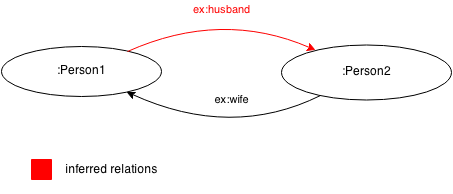
\includegraphics[width=.6\textwidth]{fig/simple-inference}
  \caption{Inference of the husband relation as inverse of the wife relation}
  \captionsetup{font={footnotesize,bf,it}}
  \label{fig:simple-inference}
\end{figure}

Many types of inferences are possible. The inference of the classes of a resource depending on a class hierarchy can be done; the example in figure \ref{fig:inference-hierarchy} shows the usage of the SORELCOM ontology to infer the classes of a resource. Combinations of different inference properties can be used to express complex relations. In figure \ref{fig:complex-inference} inverse and transitive properties together with ranges and domains, are combined to infer knowledge on a small RDF graph.

\begin{figure}[ht]
  \centering
  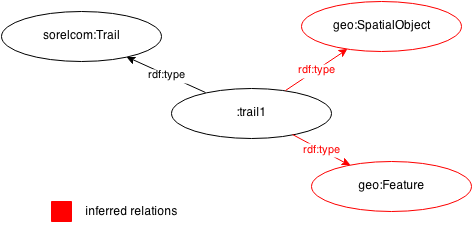
\includegraphics[width=.6\textwidth]{fig/inference-hierarchy}
  \caption{Inference of all the classes of a Trail}
  \captionsetup{font={footnotesize,bf,it}}
  \label{fig:inference-hierarchy}
\end{figure}

\begin{figure}[ht]
  \centering
  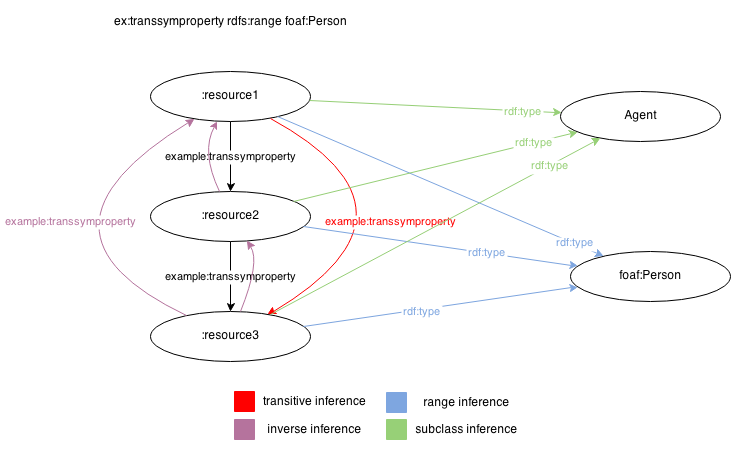
\includegraphics[width=.9\textwidth]{fig/complex-inference}
  \caption{Inference of the husband relation as inverse of the wife relation}
  \captionsetup{font={footnotesize,bf,it}}
  \label{fig:complex-inference}
\end{figure}

Depending on the describing language used, it is possible to create very complex rules, and the inference engine will automatically process all of them. This is one of the biggest advantages over relational database systems where a high amount of relations would need to be defined to encode the complex relations that can be represented in a ontology based system and allows to build complex queries.

\subsubsection{Schema and data separation and reusability}

Ontologies provides mean for reusing other data models, since it is possible to import ontologies into another one. This way, it is possible to use already defined concepts without the need to develop vocabularies for them. One example of this can be found in the SORELCOM vocabulary, where the FOAF, GeoSPARQL, DC and W3C media ontologies are reused.

Besides, this allows separation between the data model and the actual data. In relational database management systems, the structure of the data is physically created on the system itself (for example, a file for each table) and it is not fully supported to import the model of one database to another. When using ontology based databases, the data model is represented by a ontology which can be imported into any data store, thus it is possible to reuse the schema among several different databases.

\subsubsection{Linked Open data}

Ontologies are a tool that facilitate the publishing of Linked Open Data. The inference mechanisms used on these ontologies are not so relevant in this case, however the concepts expressed are crucial. Ontologies allow reusing other vocabularies to express the data model, which is a key point when developing a linked model.

Linked data refers to a set of best practices to publish and interlink structured data for access by both humans and machines via RDF. In order to do this it is necessary to make use of URIs as a real unique identifier, there is no point if a relation that expresses that two persons know each other has a different URI in every dataset. In order to avoid this, well known vocabularies, such as FOAF, and these concepts and relations are uniform among most if not all datasets. This is only possible when using ontology based design, for only ontologies allow this level of reusing.

\FloatBarrier

\section{Design of the central server}\label{sec:serverdesign}

\subsection*{A note on JavaScript program modeling}

All of the software implemented through the project has used JavaScript as the programming language of choice. Due to the single-threaded nature of the JS runtimes, most of the JavaScript programming is done asynchronously. 

In addition, the language is not strictly object oriented (although it can be used in that way), however, JS programming paradigms and platforms have tried to bring structure by using modular approaches.

Due to this, there are some considerations to take into account in the class diagrams presented in the following sections.

First, the classes represented are not always classes in the strict sense. Many times these classes are tagged as \textit{services}, \textit{controllers} or \textit{factories} since they follow the pattern of some framework. Even if they are not strictly classes, they behave in very similar ways and they can be represented with the same relations.

Second, in JavaScript most of the data manipulated is an Object , even functions. These objects act as name/value dictionaries. Due to this, it is not necessary to define classes when the object only requires data manipulation and has no operation associated, unlike in object oriented languages such as Java. What would seem as a poor decision choice in other languages (dictionaries instead of classes) is the standard way of working in JavaScript.

Finally, due to the asynchronous nature of the programming envirnoments, the event-oriented programming model is followed. This consist on passing callbacks as parameters to functions, which will be executed when the operations are done (see chapter \ref{ch:implementation} for more details). Due to this, it is usual to find parameters of type \textit{Function} in the modeled operations, these arguments are the event callbacks.

\subsection{Web server}

\begin{figure}[ht]
  \centering
  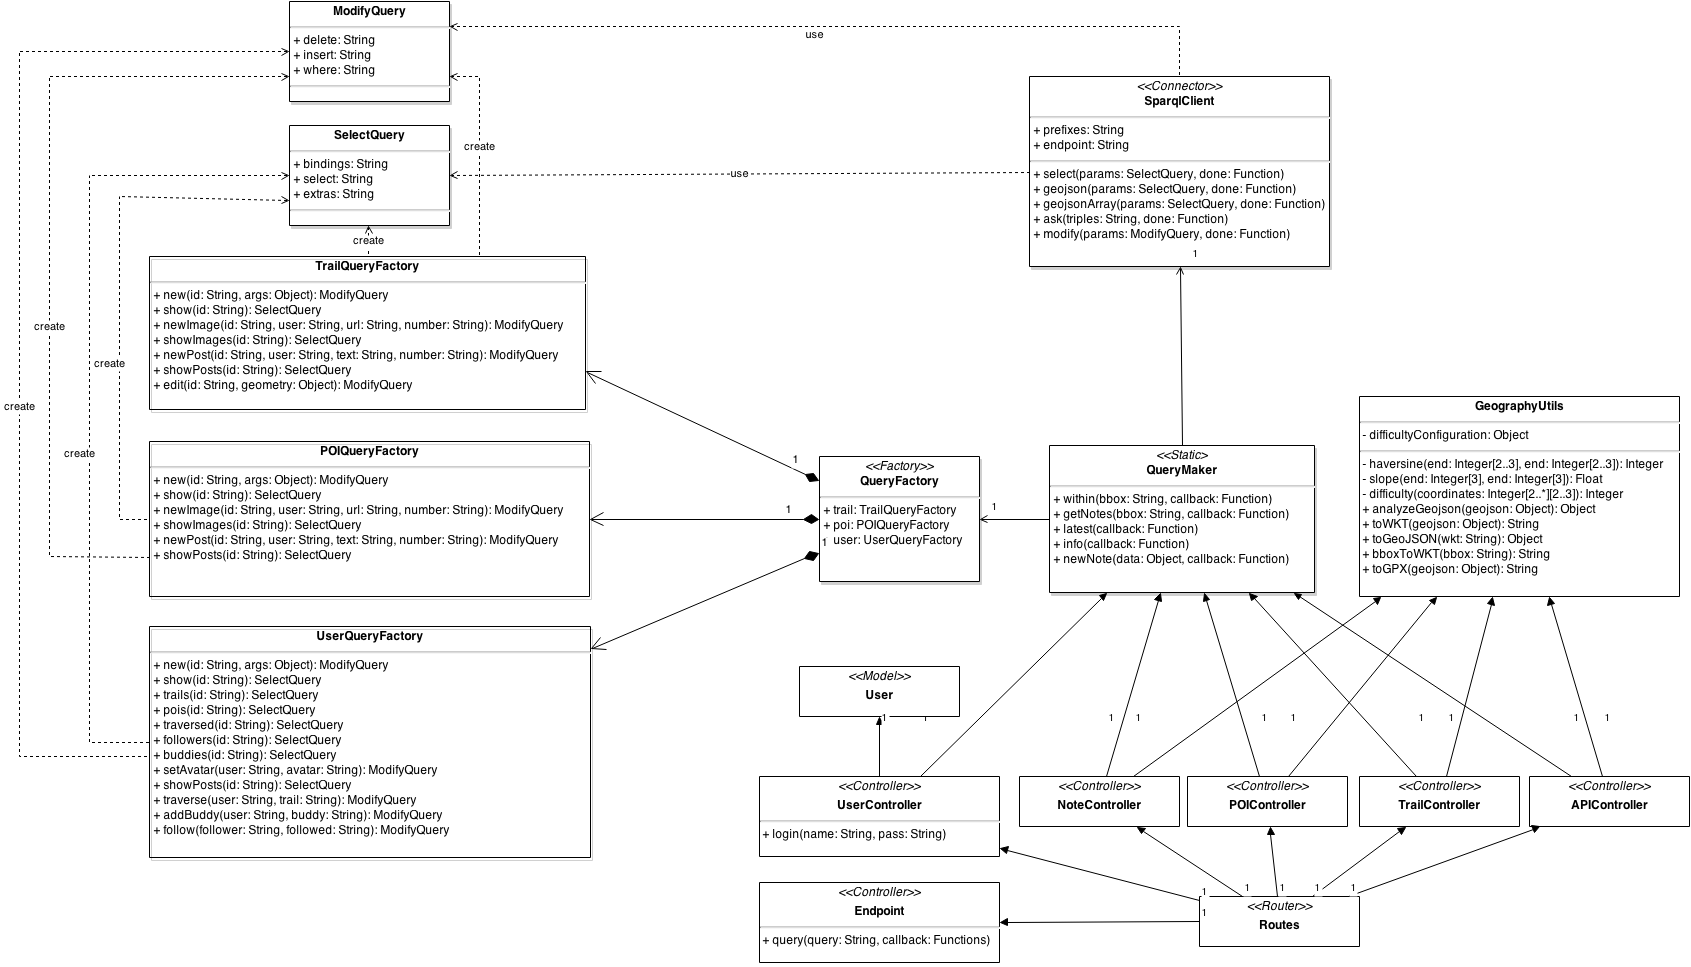
\includegraphics[angle=270,width=.8\textwidth]{fig/server-diagram}
  \caption{Class diagram of the web server}
  \captionsetup{font={footnotesize,bf,it}}
  \label{fig:server-diagram}
\end{figure}

The role of the central server is that of implementing most of the functionality of the system and acting as a mediation among the other components. It provides the client application with access to the database; it captures the data sent from the applications, transforms it to RDF and stores it in the database and it is responsible of the analysis of geographical features and of recommendations.

Figure \ref{fig:server-diagram} shows a diagram of the classes of the server. Most operations are not shown on the diagram because they are simply wrappers around other functions found on related classes. The role and relation of the classes is detailed below:

\begin{description}
\item[Routes:] This class takes care of the routing on the web server. It reads the requests and calls an adequate function depending on the specified route. It implements the REST API, detailed on section \ref{ssec:api}.

\item[Controllers:] There are several controllers present on the server. These modules are the ones implementing the functions that the router calls. Most of these functions perform some analysis or transformation on the data received, using the functions on the module \texttt{GeographyUtils} and then call the \texttt{QueryMaker} class in order to retrieve or store data from the database.

Two of the controllers differ a little from the rest. The first one is the \texttt{UserController} which makes use of a model in order to store user password hashes on a NoSQL database. It also provides authentication.

The second of these is the \textit{Endpoint} module. This controller exposes a single operation, used to route a SPARQL query to the database. This function also takes care of transforming the response of the database into a format that can be sent to the applications.

\item[\texttt{GeographyUtils:}] This module provides several utility functions used to analyze and manipulate spatial data. Most of the functions are used to obtain relevant data, for example, the \textit{haversine} operation obtains the distance between two points taking into account the spheric shape of the earth. Other functions transform between the different formats used to represent spatial data in the system, namely GeoJSON, GPX and WKT.

\item[\texttt{QueryMaker:}] The QueryMaker is the most complex class on the server. It takes care of elaborating SPARQL queries for the different functions implemented in the API.

In order to query the database the following chain is followed:

\begin{enumerate}
\item A function of the \texttt{QueryMaker} is called.
\item The query maker calls a function on the \texttt{QueryFactory} or one of its components in order to produce a Object representing the query string.
\item This object is sent to the \texttt{SparqlClient} which will form a query string and send it to the endpoint exposed by the database in a HTTP request.
\item The response is transformed into a regular JavaScript object or into a GeoJSON object.
\item The object is sent to the requester.
\end{enumerate}

\item[\texttt{QueryFactory:}] This module has the task of producing a object representing a query depending on the request done. It is related by composition to other three objects, which are just specialized factories that translate the read, write and update operations to SPARQL queries.

\item[\texttt{SparqlClient:}] It is a HTTP client for the semantic datastore. It can be initialized with a set of prefixes used to shorten the queries and with the URL of a endpoint. The task of this object is to transform the \texttt{SelectQuery} and \texttt{ModifyQuery} items received into SPARQL query strings, sending them to the database and then parsing the response into an adequate format.
\end{description}

\FloatBarrier

\subsection{REST API}\label{ssec:api}

The API on the severs is designer following the REST (Representational State Transfer)\cite{rest} style. This style is characterized for the following:

\begin{itemize}
\item The server and the client are stateless, all the information needed to give a response is provided in the request. This is not always completely followed, due to the use of cookies. however, some of the practices, for example URL rewriting, are unacceptable in REST.
\item Information on the system is exposed as resources which have well defined operations.
\item There is a universal syntax for resource identification, each resource is only available through its URI.
\end{itemize}

The advantages of using REST over other approaches to API styling are various. First, since there is no state to be maintained on client or server, the server scales more easily. In addition, it is possible to provide links to the operations of the object in the API responses, to make the automatic analysis and usage of the API possible.

The graph in figure \ref{fig:api-diagram} represents the resources and operations exposed by the API.

\begin{figure}[ht]
  \centering
  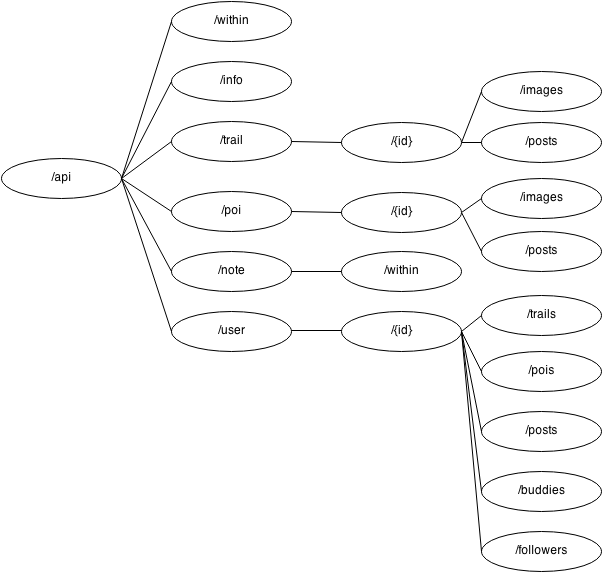
\includegraphics[width=.8\textwidth]{fig/api-diagram}
  \caption{Resources and operations of the API}
  \captionsetup{font={footnotesize,bf,it}}
  \label{fig:api-diagram}
\end{figure}

The responses given by the API are JSON objects. This choice is made on the basis that JSON objects are faster to send over a network than other formats such as XML files. In addition, JSON is usually deemed as easier and faster to parse than XML. When sending spatial object, these JSON objects are formatted to follow the GeoJSON standard (see section \ref{sec:geojson}).

\subsection{Data agregator}

In order to build a truly linked data application, it is necessary to extract knowledge from the different datasets around the web. Two services have been used to obtain information, OpenStreetMap and Geonames.

OpenStreetMap is a initiative which aims to create and provide free geographic data from around the world. It is a completely collaborative initiative, so all the data is user generated, which may cause inconsistencies in a few occasions.

Geonames is a geographical database which is available for free download under the creative commons license. It consist of over 8 million features from around the world, which provides high performance services. It server more than 30 million web service requests per day.

Both applications provide two ways of accessing their data. The first of them is downloading this data in a file, but they also provide APIs to access different functions.

The platform uses the APIs of these services to access the data. This is done in order to automate the data access and enable the update of the data every period of time without the need for a manual download.

OpenStreetMap provides two different APIs. One of them is optimized for writing operations, while the other ones offers read only functionality. This platform receives data from the Overpass API, which allows for complex queries over large areas.

The Geonames API is read only, however it offers additional functionality such as geocoding and reverse geocoding. It also exposes a set of feature codes which identify the types of features on the database. The API is queried using solely the feature codes for the categories which are relevant to the application.

The updates are run in a script independant to the rest of the server and works following a set of steps:

\begin{itemize}
\item For every desired category a request is made to the URL of the API.
\item The response is parsed and the features are extracted.
\item The features are transformed to the format specified on the ontology. The OpenStreetMaps taxonomy is followed to specify the category.
\item The response is checked to see if there are additional pages that the server could not send due to size constraints.
\item If there are more pages to query, the process is repeated.
\end{itemize}

At the current time, the queries are specific to the region of Spain. This is because it would be unreasonable to expect to have a database that can handle features from the whole world in such small development time.

\subsection{Socket server}

In order to provide real time communication with the mobile application, the server needs another component. For this, a socket server has been designed, which will establish permanent connection between the server and the client.

The diagram of the socket server is shown in figure \ref{fig:socket-component}.

\begin{figure}[ht]
  \centering
  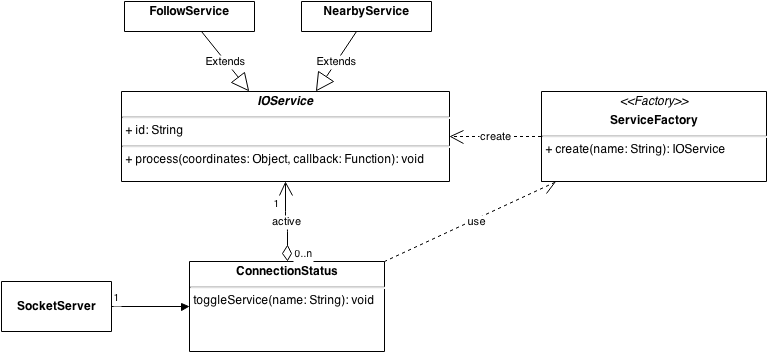
\includegraphics[width=.8\textwidth]{fig/socket-component}
  \caption{Socket server class diagram}
  \captionsetup{font={footnotesize,bf,it}}
  \label{fig:socket-component}
\end{figure}

\begin{description}
\item[Socket server] The socket server is a process separate from the web server that runs on the same machine. This server takes care of establishing permanent connections with the mobile clients that which to use the real time services.

\item[Connection status] Each connection needs to keep track of an status, that is, the services it is subscribed to and the option configuration for those services. Through the status, a client can subscribe to different services.

\item[Services] Services in the socket server are functionalities offered by the platform. One of such services can be dedicated to tracking the features near the user or to follow a certain trail.
\end{description}

The server takes care of receiving messages from the client in the form of coordinates and calling the processing function of every service to which the user is subscribed. This is done following a protocol specified in section \ref{sec:mobileappdesign}. The sequence diagram for this functionality is shown in figure \ref{fig:socket-flow}.

\begin{figure}[ht]
  \centering
  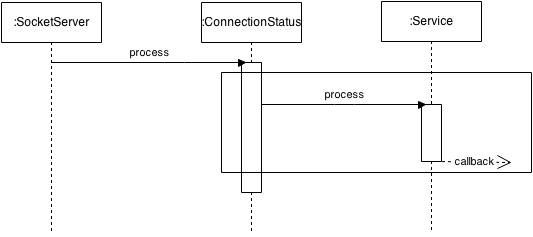
\includegraphics[width=.8\textwidth]{fig/socket-flow}
  \caption{Service processing sequence diagram}
  \captionsetup{font={footnotesize,bf,it}}
  \label{fig:socket-flow}
\end{figure}

\FloatBarrier
\section{Design of the web application}\label{sec:webappdesign}

The design of the web application has been highly influenced by the framework of choice, AngularJS, (see section \ref{sec:angular}). This framework does not only provide a structure to a project, it imposes it. The architecture of the application is thus conditioned by this tool, which is why many classes appear as controllers, services or factories; all of them patterns widely used on Angular applications.

The web application gives the user access to the following actions:

\begin{enumerate}
\item Register on the platform
\item Log in
\item Browse through the features and users of the application
\item View details about features and users
\item Upload a trail or point of interest
\item Draw a trail on a map
\item Mark a point of interest in a map
\item Edit a trail in a map
\item Explore the world through a map
\item Upload images to a feature
\item Comment on a feature
\item Follow or add a user as a buddy
\end{enumerate}

Figure \ref{fig:webapp-components} provides a high-level overview of the components that form the web application and the way they depend on each other. 

\begin{figure}[ht]
  \centering
  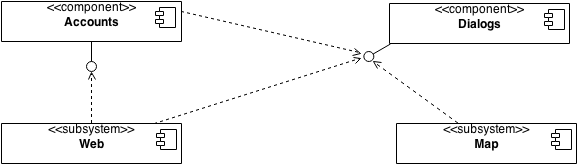
\includegraphics[width=.8\textwidth]{fig/webapp-components}
  \caption{High-level view of the web application components}
  \captionsetup{font={footnotesize,bf,it}}
  \label{fig:webapp-components}
\end{figure} 

\begin{description}
\item[Dialogs:] Provides the other components with utilities for user interactions. These take form of UI dialogs that allow the user to log in, to load files, etc.
\item[Accounts:] Implements the functionalities needed to log the user in, to register new users and to store locally the information about the users, to avoid excessive requests to the server.
\item[Web:] Most of the user interface is implemented in this component. It is a subsystem that contains the views and the functionality needed to browse the information on the server.
\item[Map:] The map provides the application with a interactive map which allows to explore the trails and points of interest of the world and provides access to the functions of the editor.
\end{description}

In addition to these components, an API service is defined and used through all the components to access the server. 

\subsection*{AngularJS notations}

Before describing the internal design of the different components it is necessary to give some notes about how AngularJS structures applications.

\begin{description}
\item[View:] It the context of this framework, a view is an HTML document, enhanced with directives that allow it to access data.
\item[Controller:] The controllers contain the functionality needed to manipulate the view. The data shown on the HTML documents and the functions used are stored on the controllers.
\item[Scope:] Named \texttt{\$scope} in the framework, the scope is a object that binds the view and the controller. The view does not have access to the controller directly, it accesses the scope, thus, when the controllers want to expose information it needs to save it in the scope.
\item[Model:] A model is any kind of domain related data on the server. It is usually obtained through REST APIs.
\item[Service:] Services are objects defined for a particular application which can be reused through all the controllers. They are used for data sharing, code reuse, etc. There are several types of services. The most common one used is the plain service pattern, which exposes a singleton object. Since most of the services follow the singleton pattern, it is not explicitly noted on the class diagrams.
\item[Factories:] Factories are a type of service. The difference with the regular services is that factories just expose a set of functions, they cannot be used to share data. On the other hand they are simpler to implement than regular services.
\end{description}

\FloatBarrier
\subsection{API connector}

Figure \ref{fig:api-component} provides a class diagram showing the API connector and the object it creates, which represent the data model on the application. 

\begin{figure}[ht]
  \centering
  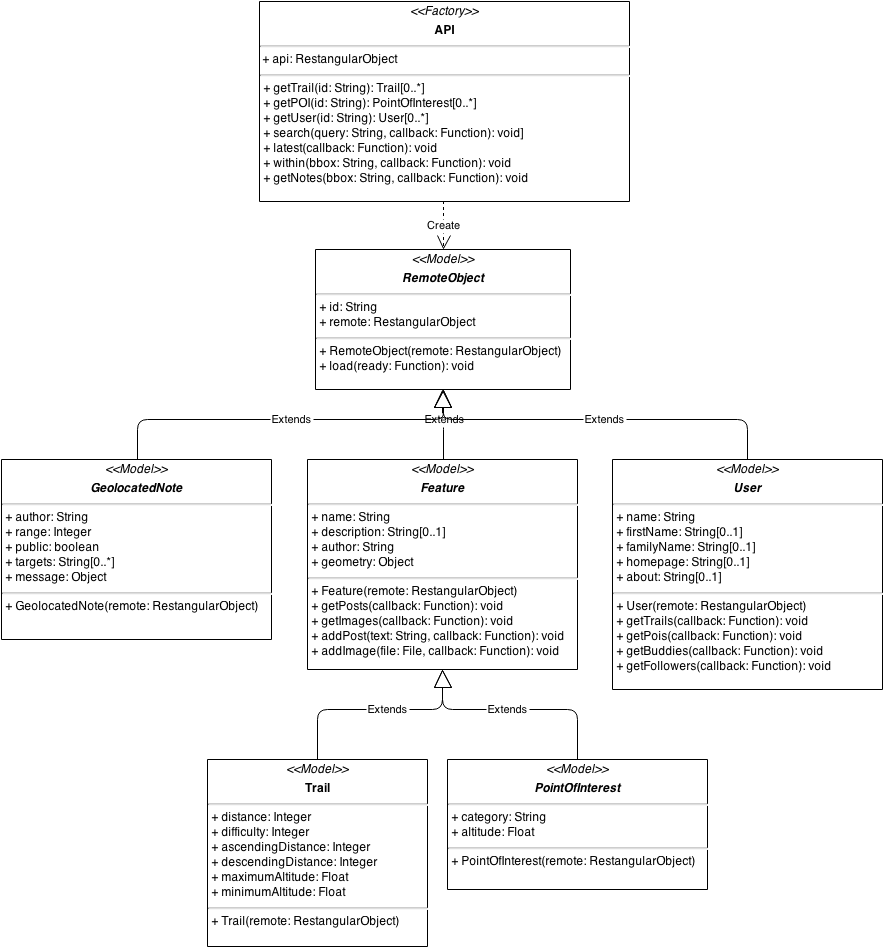
\includegraphics[width=.85\textwidth]{fig/api-component}
  \caption{API connector class diagram}
  \captionsetup{font={footnotesize,bf,it}}
  \label{fig:api-component}
\end{figure}

It is noteworthy to mention how the models in the system work. Since all the data is extracted from the server in a asynchronous way, there is a need to register an event in order to know when the data has arrived from the server. The objects in the model are created as soon as the remote call to the server is done. Then a callback is registered via the \texttt{load} method, which specifies how the object will be read and it's data populated.

This way it is possible to bind the data to the views immediately without needing to wait for these object to be populated. Below the role of each class is explained:

\begin{description}
\item[API object] The API class exposes an object that can be used to access the API of the server. This object is obtained from the Restangular module and it provides a way to navigate REST API and query them using the different HTTP methods.

In addition, convenience methods which create and return model objects are provided.

\item[RemoteObject] It is the superclass of all models obtained from the server. It contains an id, which is a string representing the URI of the resource and a object that allows to query this URI with different HTTP methods.

\item[User] It represents the users of the application. Users are identified by both their username and their email. The trails and points of interest added, as well as trail buddies and followers.

\item[Feature] Features are the trails and points of interest on the system. Each of them contains data specific to the type of feature it is, but all allow to access the media and the posts on them.

\item[GeolocatedNote] These objects represent the geolocated notes of the systems. The difference with features is that they do not contain posts and media is treated differently, for it is the main content.
\end{description}

\FloatBarrier
\subsection{Web}

Figure \ref{fig:browse-component} shows the class diagram for the web subsystem. This component contains the views and the functionality needed to browse through the information on the platform. The subsystem consists solely on a series of views controllers which make use of the API and dialogs.

\begin{figure}[ht]
  \centering
  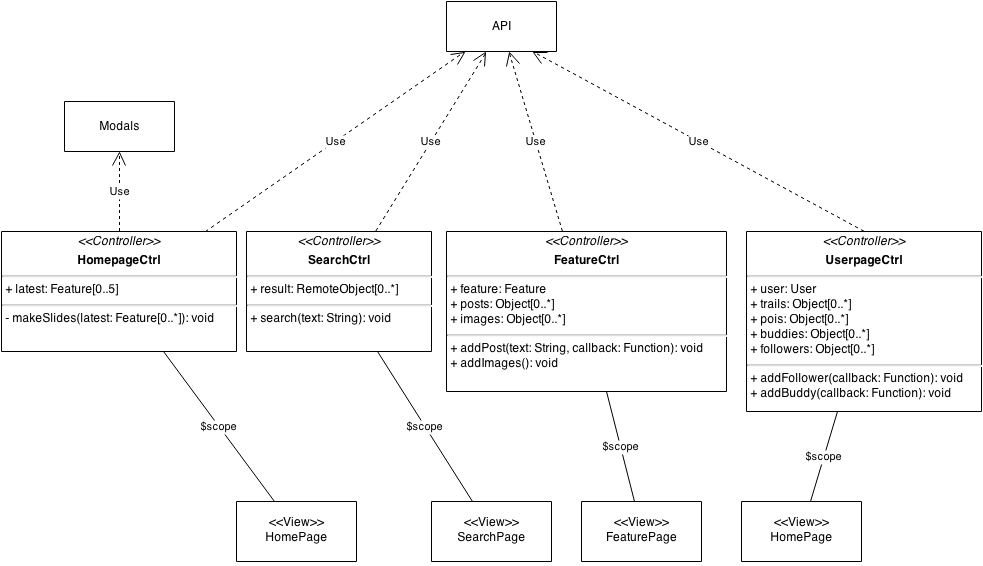
\includegraphics[width=.8\textwidth]{fig/browse-component}
  \caption{Web subsystem class diagram}
  \captionsetup{font={footnotesize,bf,it}}
  \label{fig:browse-component}
\end{figure}

\begin{description}
\item[Home page] It is the first page that a new user will find when entering the platform. It shows some guidelines on how to use the application and provides information about the latest changes on the platform.

\item[Search page] It allows the user to perform text based search on the platform. The retrieved information will adapt its display to the type of resources found. The search takes into account not only the content on the resources but also related resources, however, only trails, points of interest and users are displayed.

\item[Feature page] It offers a detailed view of the features on the platform and the related information. If provides a map to view the geographic information of the features and allow to create posts.

\item[User page] It offers an overview of the users on the platform. It allows to see the information that a user has shared on the page and provides a way of following and adding users as buddies.
\end{description}

All the views in the subsystem contain a navigation bar which allows to log in, register and browse in addition to give quick access to the subsections of the page.

\subsection{Map}

Figure \ref{fig:map-component} shows the class diagram for the web subsystem. It provides a interactive map through which features on the world can be viewed and trails can be edited.

\begin{figure}[ht]
  \centering
  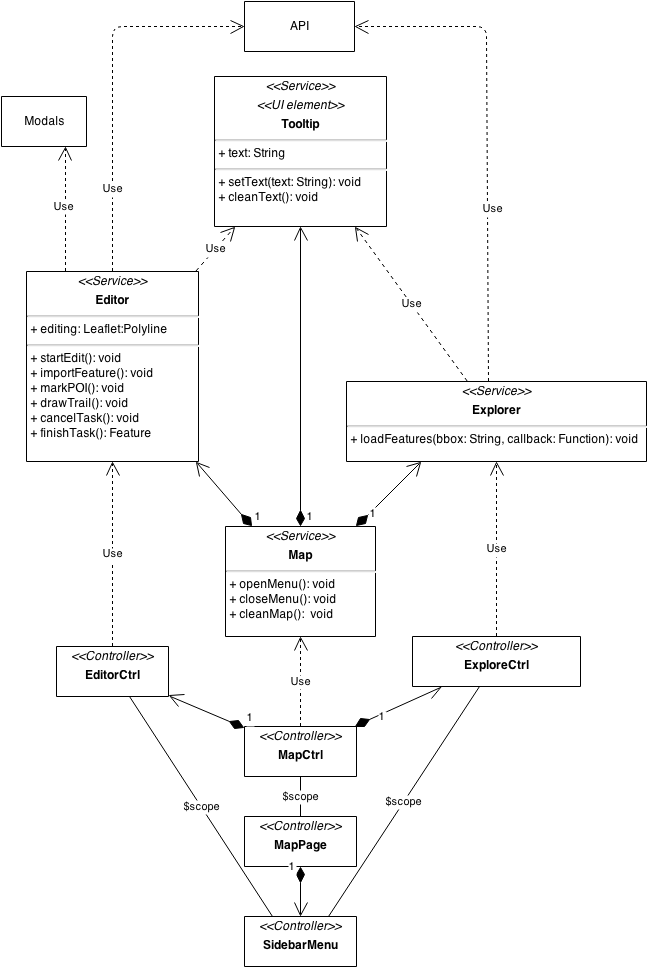
\includegraphics[width=.75\textwidth]{fig/map-component}
  \caption{Map subsystem class diagram}
  \captionsetup{font={footnotesize,bf,it}}
  \label{fig:map-component}
\end{figure}

\begin{description}
\item[Map] The map view provides a map which takes the whole space on the browser. A sidebar menu contains the needed elements to access the functionality of the component. This sidebar provides the editor and the explorer which are build at components of the map view.

\item[Explorer] The explorer does not provide any direct functionality, however, while this view is active the controller takes care of retrieving information about features that can be found on the current viewport of the map.

\item[Editor] The editor provides functionality to upload and modify routes and points of interest. All this is done through a point and click interface on the map.
\end{description}

The map is built as a service, in order to be able to share the map element through all the controller that access it. The editor and explorer functionality and data are all contained in their own services which are accessed by the respective controllers.

In addition, a \texttt{Tooltip} service is provided which is represented on the map view. It shows information about the current action being taken by the user, such as editing a trail. It acts as a tutorial.

The map works making use of the Leaflet framework. Since the API responds using GeoJSON when querying for spatial data and the library supports direct representation of this format on the map, adding data to it is straightforward. The Leaflet map is contained in the \texttt{Map} service and it is accessible by both the editor and the explorer. These two classes however include their own data on the map and must make sure that when the controller is changed the data created by these classes is cleaned from the map. This is done by the controllers themselves, which register and function that destroys the data on the map when the controller is destroyed.

Most of the functionality on the map is done through the registration of events. For the exploring of the world, a request is done to the server every time the user zooms or moves the map. For the drawing of routes and marking of points of interest, an event is registered for clicks on the map. This way is how the interaction with the user is provided in the application, by registering callbacks for the actions it does.

\subsubsection*{Trail edition}

Most of the functionality of the map can be implemented using the events and utilities provided by the leaflet framework. The edition of trails however is a task that has a high complexity related.

In order to provide this functionality, a Leaflet plugin has been developed to create editable trails. Trails are represented as polylines in a map. These polylines are lists of coordinates that are represented in a map by the lines that join them. Editing a trail implies moving these coordinates, which is not supported by default in Leaflet.

There are several plugins already developed which allow this editing, however, they all suffer from the same problem which is performance. Most of this solutions add draggable markers to the coordinates of the line, which results in a lack of performance when there are more than around 200 points. In order to avoid this, the plugin has been developed to show only a limited number of markers, which is necessary considering that trails usually have over 500 points.

Detail about the implementation of this plugin can be found on chapter \ref{ch:implementation}.

\FloatBarrier
\subsection{Accounts}

Figure \ref{fig:accounts-component} shows the class diagram for the accounts component. It provides the functionality needed to register and authenticate users as well as storing the loged user locally to avoid excessive queries to the server.

\begin{figure}[ht]
  \centering
  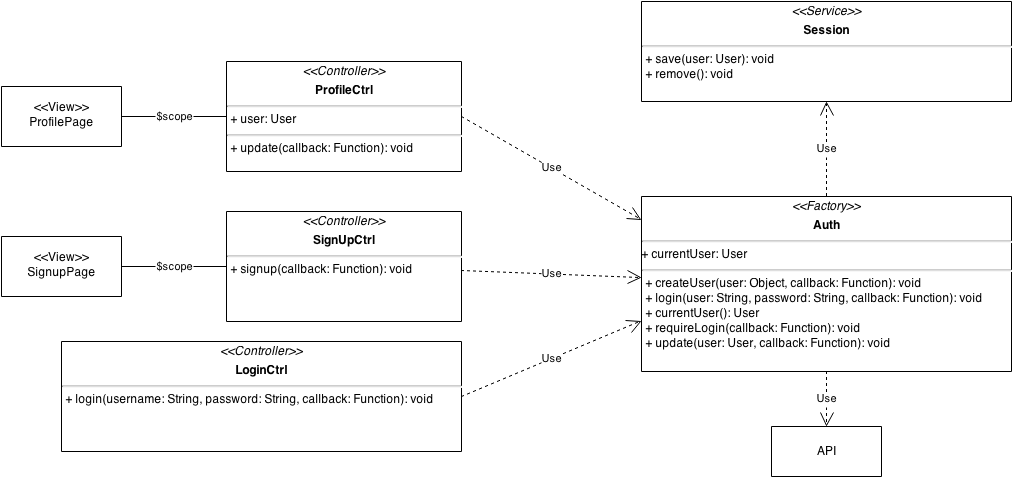
\includegraphics[width=.8\textwidth]{fig/accounts-component}
  \caption{Accounts component class diagram}
  \captionsetup{font={footnotesize,bf,it}}
  \label{fig:accounts-component}
\end{figure}

\begin{description}
\item[Profile] The profile allows a user that is already logged in to view his own profile and to change his preferences and personal data.
\item[Sign up] The sign up page allows a person to register as a user in the platform. The information needed for registering is only a user name, a email and a password. Once registered it is possible to add additional information through the profile page. 
\item[Login] The log in controller is not associated to any view in this diagram for it is used by the dialog system. This is because login may be required in several parts of the application and it is more convenient for the user to have it offered as a modal.
\item[Auth] It is a service used through all the platform that allows to query the currently logged user, to ask for updates on his information and to log in and register.
\item[Session] A wrapper over the HTML5 SessionStorage API, which is used to store locally the information of the user once logged in.
\end{description}

\FloatBarrier
\subsection{Dialogs}

Figure \ref{fig:dialogs-component} shows the class diagram for the dialogs component. This component provides utilities to facilitate user interaction in the form of dialogs that give access to various functionalities used across the system. 

\begin{figure}[ht]
  \centering
  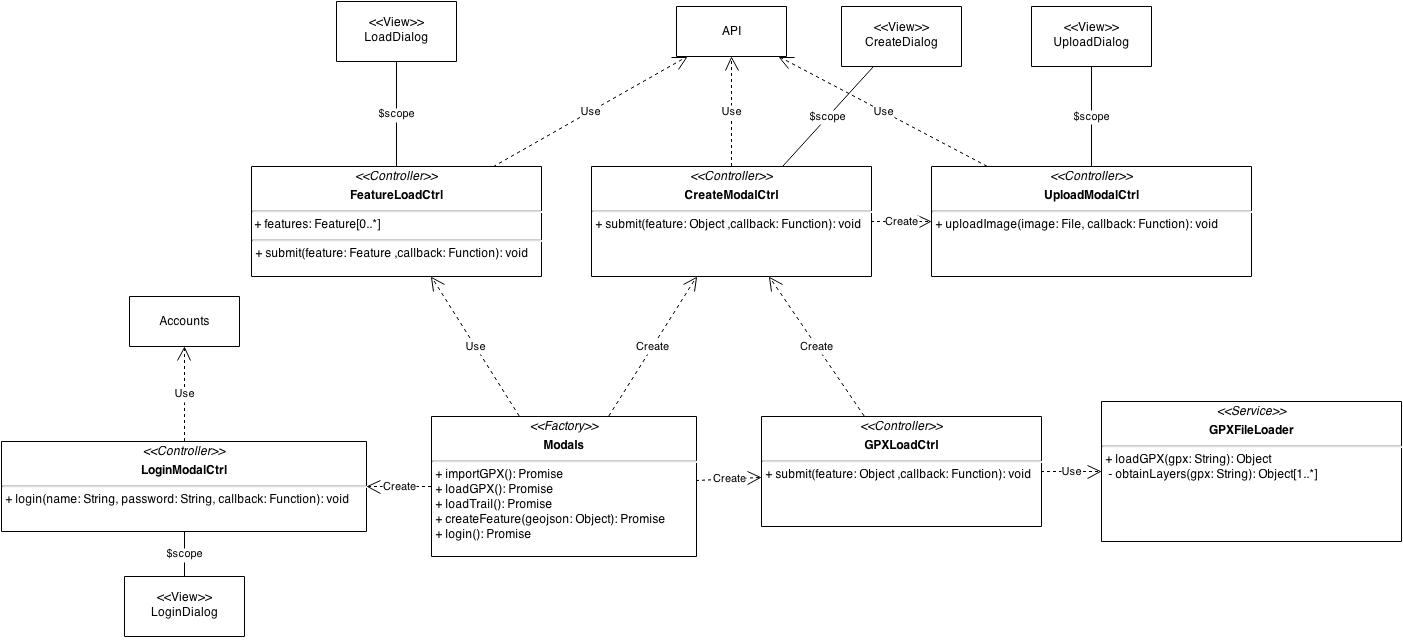
\includegraphics[width=.8\textwidth]{fig/modals-component}
  \caption{Dialog component class diagram}
  \captionsetup{font={footnotesize,bf,it}}
  \label{fig:dialogs-component}
\end{figure}

\begin{description}
\item[Log in] The log in dialog provides a very simple interface for the users to log in to the platform. It requires an email and a password for the authentication.
\item[Feature load] The loading dialog allows downloading trails from the server. It is used on the editor to select a trail to edit.
\item[Feature creation] The feature creation dialog provides a form to create points of interest or trails. It is used after loading a GPX file or marking the feature on the mark. Once the feature is saved, it calls the upload dialog which allows the uploading of images to the platform.
\item[GPX loading] This dialog provides functionality for loading a GPX file. It analyzes the contents of the file using the \texttt{GPXLoader} service and provides an interface for the user to chose one of the features contained in the file. Once the feature is selected the creation modal will be used in order to obtain the data about this feature.
\end{description}

The \texttt{Modals} class exposes all the functionality listed, thus, it is the interface through which other components can invoke the dialogs. In essence, this class provides shortcuts for creating dialogs and returns \texttt{Promises}, objects that are notified when the modal is closed.

\FloatBarrier
\subsection{Graphical design}

The graphical design of a web application is sometimes as important as the logical design and implementation of it. Web pages are usually created to be used by a wide array of users, whether they are tech savvy, they can handle a computer or not. In addition, many different devices have to be able to access the applications, which is also something to take into account when creating the interface.

\subsubsection*{Responsive web design}

Responsive web design is an approach to web design which aims to provide optimal viewing experience across a wide range of devices. It is not just about providing a uniform easy to read interface, it has to respond gracefully on every device, optimizing its view for the screen on which it is being displayed \cite{rwd}.

This can be achieved with a series of techniques. Fluid grid layouts are used to reposition elements depending on the size of the screen on which the document is displayed. Responsive graphics are used in order to achieve uniform views through all viewport sizes.

The CSS3 technology supports this design approach with the use of media queries. These constructs allow to specify a output type such as a printer or a screen and a viewport size (width and height). An example of the usage of media queries can be found in listing \ref{lst:mediaquery}.

\begin{listing}[ht]\centering
  \begin{minipage}{.6\textwidth}
    \begin{minted}[linenos=true,mathescape,gobble=6]{css}
	     @media (min-width: 481px) and (max-width: 768px){
	       /** Styles for the specified viewport */
	     }
	     
	     @media screen and (min-width: 780px){
	       ..
	     }
    \end{minted}
  \end{minipage}
  \caption{CSS3 media query example.}\label{lst:mediaquery}
\end{listing}

In addition to media queries, the CSS3 framework Twitter Bootstrap \cite{twitterbootstrap} has been used to create a responsive application. For this, the framework provides a series of responsive elements, for example, navigation bars which hide their buttons on a submenu when the screen is not big enough. However, the most important element provided by this framework is its grid system, which allows to structure the contents of a web page on different ways depending on the type of screen (desktop, tablet or mobile).

This tool together with custom responsive style sheets has been used to build an application that can be displayed effectively in many devices. An example of this behavior can be found on figure \ref{fig:responsive}, which depicts how the map interface adapts to different devices.

\begin{figure}[ht]
  \centering
  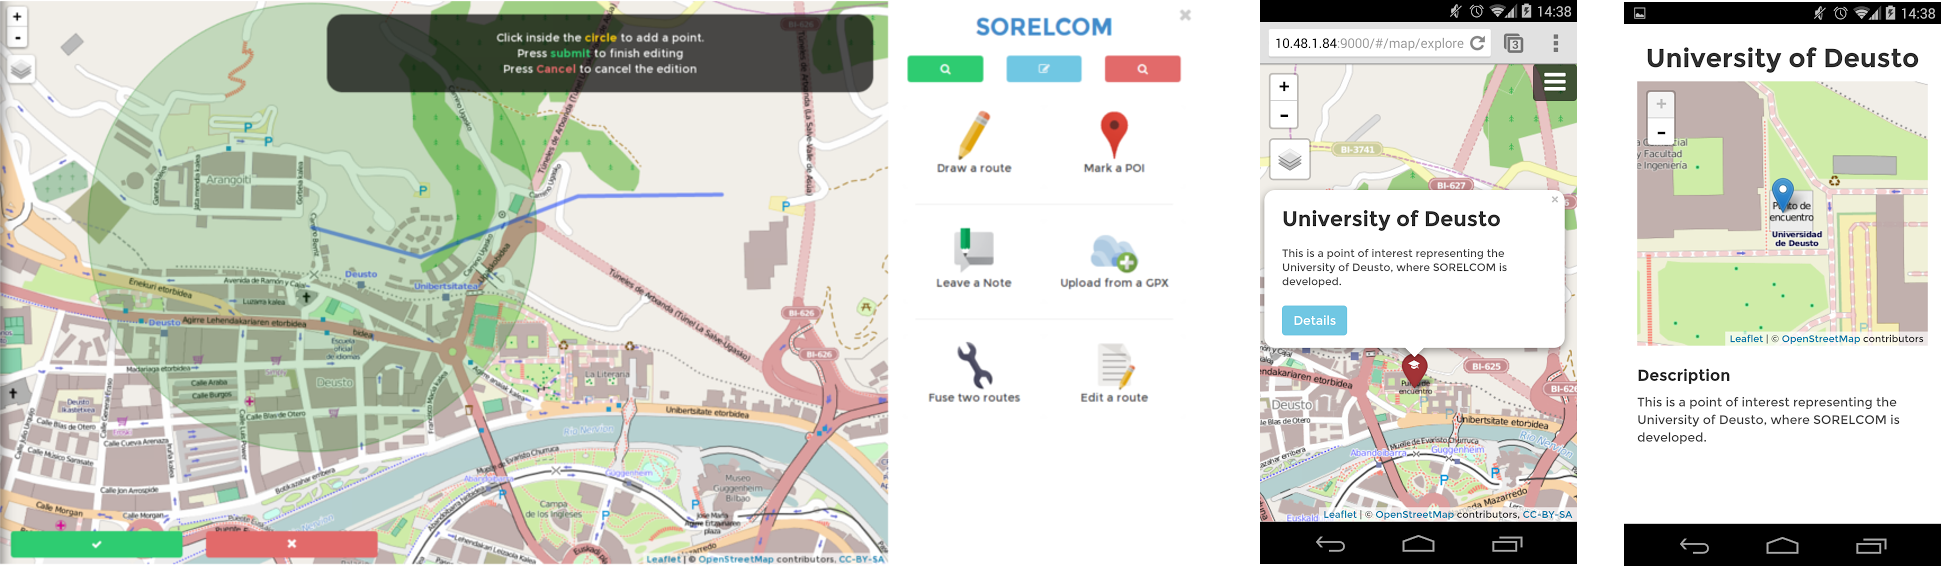
\includegraphics[width=.8\textwidth]{fig/responsive-example}
  \caption{Responsive web design on SORELCOM}
  \captionsetup{font={footnotesize,bf,it}}
  \label{fig:responsive}
\end{figure} 

\subsubsection{Mobile first}

When designing a responsive application, the usual train of thought it to think on the structure the interface will follow on desktop devices and then transform it to mobiles and tablets. When following a mobile first approach, contents are designed to be displayed in mobile first and then adapted to tablets and desktop devices.

However, mobile first design implies more that just interfaces. Some platforms offer different URLs for their mobile and desktop versions, however, this causes loss of visibility in search engines, mobile first approaches discourage this practice. 

Single pages applications can also be used for mobile first design. The downloading and displaying of a web page takes more time in mobile devices compared to more powerful computers which can be a real issue. SPAs load the document only once and then change the views of the interface using AJAX, resulting in a faster and more fluid execution.

\FloatBarrier
\section{Design of the mobile application}\label{sec:mobileappdesign}

The mobile application has been developed using the HTML5 development framework Phonegap. Due to this, it has been possible to reuse most of the existing functionality from the web application. In fact, the mobile application is structured the same way as the web and uses the same frameworks and libraries.

Most of the components of the web application have been included, with the exception of the map editor. The dialogs of the web application are changed to become regular views instead of pop-up elements.

The mobile application gives access to the following actions:

\begin{enumerate}
\item Register on the platform
\item Log in
\item Browse through the features and users of the application
\item View details about features and users
\item Record a trail
\item Export a trail as GPX
\item Upload a trail 
\item Receive notification about nearby features and notes
\item Mark a note on the current location
\item Follow a trail
\end{enumerate}

\subsection{Class design}

In addition, a new component is added to provide the mobile specific functionality. Figure \ref{fig:mobile-diagram} shows the structure of the new component.

\begin{figure}[ht]
  \centering
  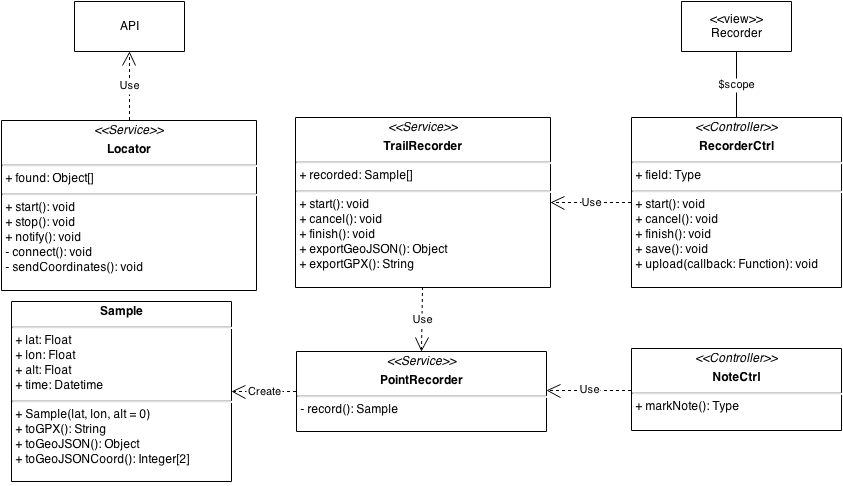
\includegraphics[width=.8\textwidth]{fig/mobile-diagram}
  \caption{Class diagram of the new components of the mobile}
  \captionsetup{font={footnotesize,bf,it}}
  \label{fig:mobile-diagram}
\end{figure} 

\begin{description}
\item[Trail recorder] The trail recorder takes care of periodically saving points by using the \texttt{PointRecorder} class. This service is used to record trails that the user is doing. Once a trail is recorded it is possible to svae it as a GPX file or to upload it to the platform.
\item[Note marker] The function of the note marker is a simple one. It makes use of the same point recorder as the trail recorder in order to mark the current location of the user and saving a geolocated note on the platform.
\item[Locator service] The locator service is in charge of various tasks. The first of them is always active, unless the user explicitly stops it and takes care of finding nearby points of interest, trails and notes and notifying the user about them. It also checks if the user is inside a route, and in that case it will notify the user when it gets out of the trail.

This component is the one handling real time communication with the server. It does so trough the use of WebSockets, however, when the operating system does not provide support for this technology is starts a timer to make periodic calls to the API, providing a pseudo real-time functionality.
\end{description}

\subsection{Real time communication protocol}\label{sec:protocol}

In order for the mobile client to be able to communicate in real time with the server, a very simple protocol has been designed. When the client wants the server to start tracking its location and sending notifications of nearby feature it will send a \textit{NEARBY} command. When the client wants the server to check if it is following a trail and not deviating it will send a \textit{TRAIL} command. The server can be in any combination of these two states at any moment.

In order to cancel any of these tracking functions, the command is sent again to the server. The \textit{STATE} command is used by the client to determine the current state of the server, in order to avoid canceling a function by accident, for example.

The server will not send data to the client by itself, it will wait for it to send its current location with the \textit{COORDS} order. In addition, the client will be able to configure some parameters such as the distance of on which points of interest are considered nearby with the \textit{CONFIG} command. A summary of the commands and their parameters is provided in table \ref{tab:protocol}.

\begin{table}[ht]
  \centering
  \caption{Real time communication protocol.}\label{tab:protocol}
  \begin{tabular}{lll}
    \toprule
      \textbf{Command} & \emph{parameters}  & \emph{result}\\
    \midrule
      NEARBY & none & toggle tracking nearby features\\
      TRACK & trail id or none & toggle following trail\\
      COORDS & latitude, longitude & response depending on states\\
      CONFIG & key, value & OK or ERROR response\\
      STATE & none & returns the state of the server\\
    \bottomrule
  \end{tabular}
\end{table}

The diagrams on figure \ref{fig:protocol1} and \ref{fig:protocol2} provide a graphical description of the usual procedures on the server. Usually, the client establishes a connection, sends either the \textit{NEARBY} or \textit{TRACK} commands, sends the configuration and starts sending coordinates at regular intervals.

\begin{figure}[ht]
  \centering
  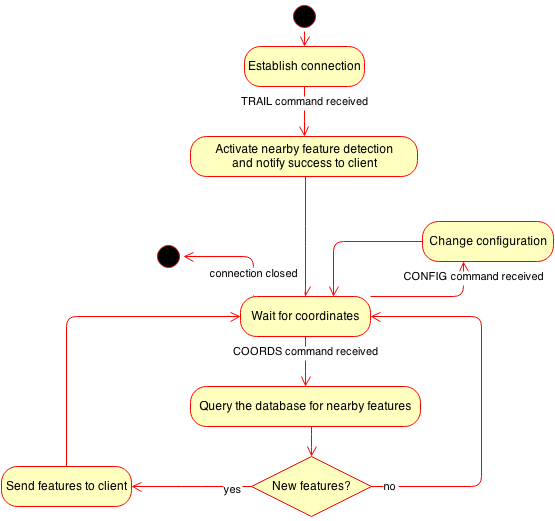
\includegraphics[width=.7\textwidth]{fig/protocol1}
  \caption{Nearby checking flow diagram}
  \captionsetup{font={footnotesize,bf,it}}
  \label{fig:protocol1}
\end{figure} 

\begin{figure}[ht]
  \centering
  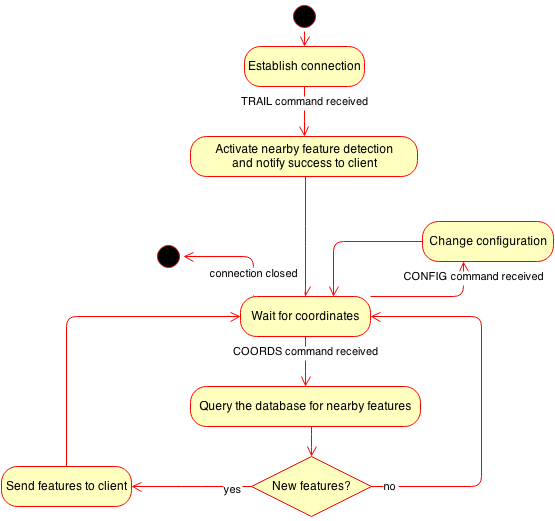
\includegraphics[width=.7\textwidth]{fig/protocol1}
  \caption{Trail following flow diagram}
  \captionsetup{font={footnotesize,bf,it}}
  \label{fig:protocol2}
\end{figure} 

These show the expected usual flow on the server, however, they are not the only possibility. It is possible to follow a trail and at the same time receive the information of nearby features. These diagrams however, do distinguish the nature of both commands. While the nearby checking functionality has a undetermined duration, it will only stop when told so or when the connection is closed; the trail functionality will stop when the user arrives at the end of the trail.

\subsection{Plugin design}

Due to the way the Phonegap library works and the required functionality, it will be necessary to create a series of background services for the application. This services need to be programmed in native language, due to this the application will initially be only developed for Android devices.

Still, a design has been created for the development of these background plugins which can be reused among different applications. This design is shown in figure \ref{fig:plugin-component}. The diagram just shows class relations and very few operations due to the possible implementation differences among different platforms. The architecture for the plugin is identical to that on the socket part of the server, for it implements the protocol to establish real time communication.

\begin{figure}[ht]
  \centering
  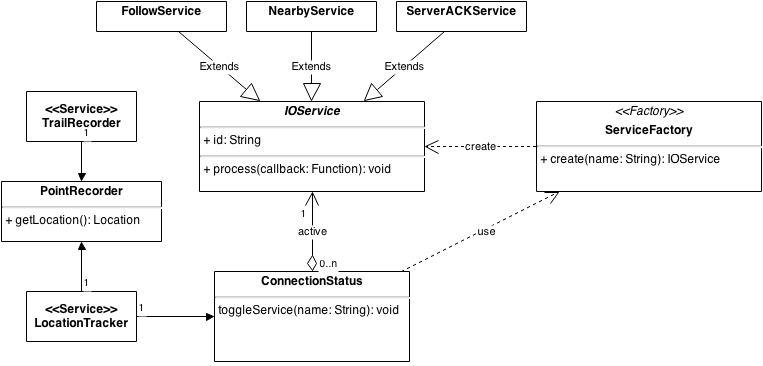
\includegraphics[width=.7\textwidth]{fig/plugin-component}
  \caption{Class diagram of the mobile application native plugin}
  \captionsetup{font={footnotesize,bf,it}}
  \label{fig:plugin-component}
\end{figure}

\begin{description}
\item[Trail recorder] The trail recorder uses the \textit{Point recorder} to access the GPS of the mobile device at regular intervals and record a full trail.

\item[Locator service] The locator is the part of the component that implements the real time communication protocol. It is designed in a identical manner to the socket server, with the difference that includes a client-only service taking care of processing the acknowledgements of the server (sent when adding or removing a service, for example).
\end{description}

The protocol described on the previous section is implemented on this component, as well as in the socket component of the server. This protocol requires to be able to add or remove services to which the user is subscribed. This is done using service identification names. When a status is asked to toggle a service it is checked if the service is already subscribed, if it is then the service is removed, if it is not then it is added.

The sequence diagram that shows this process of subscription can be found in figure \ref{fig:plugin-flow}.

\begin{figure}[ht]
  \centering
  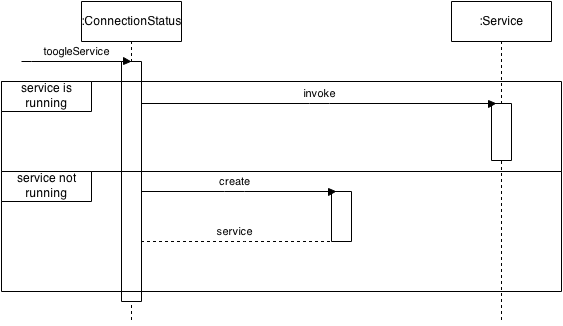
\includegraphics[width=.8\textwidth]{fig/plugin-flow}
  \caption{Service subscription sequence diagram}
  \captionsetup{font={footnotesize,bf,it}}
  \label{fig:plugin-flow}
\end{figure}

\subsection{Graphical design}

The mobile application has its appearance defined by CSS style sheets in a similar way to the web application. This, however, does not mean that the appearance of the web can be reused on the application.

Part of the application design is common to both clients, in order to keep a uniform style. Examples of this uniformity are the buttons. fonts, icons and maps used. However, the structure of the application changes radically from web to mobile clients.

Since the mobile application will only be used by smart phones which have a similar aspect ratio and screen size, it is not necessary to use responsive design at the same level. Due to this, the interfaces and the views have been adapted in order to be much more mobile friendly, sacrificing responsiveness in the process.

\FloatBarrier
\section{Development environment}

Chapter \ref{cha:research} presents a list of technologies and standards over which a initial research has been carried in order to shape the project. Still, these do not comprise the full list of technologies used on the design and development of the platform.

This section provides a list of the technologies and tools used in the realization of the project, complementing the one on chapter \ref{cha:research} and providing a brief description of each of them and their role on the project.

\subsection*{HTML5}

HTML5 (HyperText Markup Language)\cite{html5} is a core technology on the World Wide Web, used to structure and present documents. It is the fifth revision of the HTML standard, it includes semantic tags for the HTML markup language and new APIs.

Its role in this project is to define the interfaces of the clients and its APIs have been used to enhance the functionality.

\subsection*{CSS3}

CSS3 (Cascading Style Sheets) is a descriptive language used to specify the look and formatting of documents written in a markup language. It is used together with HTML in order to create visually appealing web pages. CSS3 is the third revision of this languages, which includes new style descriptors, element selectors and functionality.

It has been used in the project to define the appearance of the client applications.

\subsection*{JavaScript}

JavaScript, usually abbreviated as JS, is and interpreted programming language, based on the ECMAScript standard. It is defined as a imperative prototype based language, with weak typing. It can be considered object oriented.

It is usually used to provide interaction to web pages, which are just plain documents without JS scripts on them. Due to this, all major browser have a JavaScript runtime implemented. Even though in its origins it was purely a client-side development language, in the last years tools have appeared that allow back-end programming with this language.

It has been used to code all the logic on the developed systems.

\subsection*{SASS}

 and preprocessor for the CSS language which aims to cut on developing times and improve stylesheet maintainability. 

CSS preprocessors have become very popular lately among web developers for various reasons. First, they provide functionality that allows to programatically define styles for a web page instead of just describing, such as variables and functions. Second, these extensions improve code readability and reduce the size of the produced stylesheets. Finally, they follow the principle of DRY (dont repeat yourself), allowing to define the appearance of document without repeating directives. An example of SASS to CSS transformation can be found in figure \ref{fig:sass}.

\begin{figure}[ht]
  \centering
  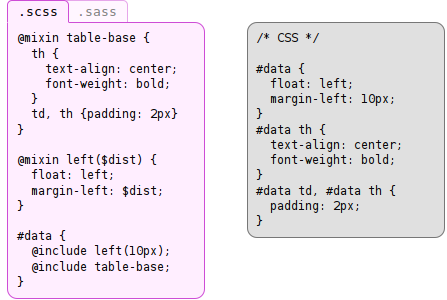
\includegraphics[width=.7\textwidth]{fig/sass}
  \caption{SASS to CSS transformation}
  \captionsetup{font={footnotesize,bf,it}}
  \label{fig:sass}
\end{figure} 

This framework has been used trough the project to create the style sheets.

\subsection*{MongoDB}

MongoDB \cite{mongodb} is a high performance NoSQL document oriented database. It is very used on Node applications due to the similarity of the documents it stores to the object of the JavaScript language. It provides APIs to work with the database using JS directly. In addition, there are node modules such as Mongoose, that provide a ORM using this backend.

MongoDB, together with Mongoose, has been used in the to store in a safe manner the sensible information of the users.

\subsection*{Passport}

Passport is a authentication framework for NodeJS (see section \ref{sec:node}). It provides secure authentication using both local account information or several APIs provided by well known services, such as Google, Facebook or Twitter.

It provides the authentication functionality on the server.

\subsection*{WebSockets}

The WebSocket protocol enables a full-duples two way communication method between a client running untrusted code and a server \cite{websocket}. It is designed to be implemented across web browsers and servers and its API is being normalized by the W3C. It provides real time communication facilities in environments in which it was impossible, that is, web applications.

It has been used to provide real time functionalities in the mobile application when the operating system allows it.

\subsection*{Socket.IO}

Socket.io is a WebSocket API that enables real-time bidirectional event base communication \cite{socketio}. It consists on two parts, a client library that runs in a browser and a server library for NodeJS, however, both have a nearly identical API.

This library uses primarily WebSockets, however, since this is a relatively new protocol and it is not implemented in every browser and device, it may fall back to other mechanisms such as AJAX polling. In addition to providing a wrapper over WebSockets, it offers several other features such as broadcasting to multiple sockets and storing data associated to each client.

\subsection*{AJAX}

AJAX \cite{ajax} (Asynchronous JavaScript And XML) is a web development technique used to create interactive applications. It allows asynchronous querying to a server, that is, requesting information without the need of updating the whole HTML document.

It has been used trough all the project to access the information on the server from the clients. In addition it is used on the mobile application to provide pseudo real-time functions when WebSockets are not supported.

\subsection*{UML}

The Unified Modeling Language (UML) is a general-purpose visual modeling language used to specify, visualize, construct and document the artifacts of a software system. It is used to capture decisions and provide understanding of the architecture and class design of the system \cite{uml}. 

UML can be used to capture information about the static design and dynamic behavior of the system and its components through different types of diagram. It is a standard used and accepted worldwide, thanks to which it can be used to expose and interchange information about system designs.

All the component and class diagrams presented in this document have been modeled according to UML standards.
